
%% bare_conf.tex
%% V1.3
%% 2007/01/11
%% by Michael Shell
%% See:
%% http://www.michaelshell.org/
%% for current contact information.
%%
%% This is a skeleton file demonstrating the use of IEEEtran.cls
%% (requires IEEEtran.cls version 1.7 or later) with an IEEE conference paper.
%%
%% Support sites:
%% http://www.michaelshell.org/tex/ieeetran/
%% http://www.ctan.org/tex-archive/macros/latex/contrib/IEEEtran/
%% and
%% http://www.ieee.org/

%%*************************************************************************
%% Legal Notice:
%% This code is offered as-is without any warranty either expressed or
%% implied; without even the implied warranty of MERCHANTABILITY or
%% FITNESS FOR A PARTICULAR PURPOSE! 
%% User assumes all risk.
%% In no event shall IEEE or any contributor to this code be liable for
%% any damages or losses, including, but not limited to, incidental,
%% consequential, or any other damages, resulting from the use or misuse
%% of any information contained here.
%%
%% All comments are the opinions of their respective authors and are not
%% necessarily endorsed by the IEEE.
%%
%% This work is distributed under the LaTeX Project Public License (LPPL)
%% ( http://www.latex-project.org/ ) version 1.3, and may be freely used,
%% distributed and modified. A copy of the LPPL, version 1.3, is included
%% in the base LaTeX documentation of all distributions of LaTeX released
%% 2003/12/01 or later.
%% Retain all contribution notices and credits.
%% ** Modified files should be clearly indicated as such, including  **
%% ** renaming them and changing author support contact information. **
%%
%% File list of work: IEEEtran.cls, IEEEtran_HOWTO.pdf, bare_adv.tex,
%%                    bare_conf.tex, bare_jrnl.tex, bare_jrnl_compsoc.tex
%%*************************************************************************

% *** Authors should verify (and, if needed, correct) their LaTeX system  ***
% *** with the testflow diagnostic prior to trusting their LaTeX platform ***
% *** with production work. IEEE's font choices can trigger bugs that do  ***
% *** not appear when using other class files.                            ***
% The testflow support page is at:
% http://www.michaelshell.org/tex/testflow/



% Note that the a4paper option is mainly intended so that authors in
% countries using A4 can easily print to A4 and see how their papers will
% look in print - the typesetting of the document will not typically be
% affected with changes in paper size (but the bottom and side margins will).
% Use the testflow package mentioned above to verify correct handling of
% both paper sizes by the user's LaTeX system.
%
% Also note that the "draftcls" or "draftclsnofoot", not "draft", option
% should be used if it is desired that the figures are to be displayed in
% draft mode.
%
\documentclass[10pt, conference]{IEEEtran}
% Add the compsocconf option for Computer Society conferences.
%
% If IEEEtran.cls has not been installed into the LaTeX system files,
% manually specify the path to it like:
% \documentclass[conference]{../sty/IEEEtran}





% Some very useful LaTeX packages include:
% (uncomment the ones you want to load)


% *** MISC UTILITY PACKAGES ***
%
%\usepackage{ifpdf}
% Heiko Oberdiek's ifpdf.sty is very useful if you need conditional
% compilation based on whether the output is pdf or dvi.
% usage:
% \ifpdf
%   % pdf code
% \else
%   % dvi code
% \fi
% The latest version of ifpdf.sty can be obtained from:
% http://www.ctan.org/tex-archive/macros/latex/contrib/oberdiek/
% Also, note that IEEEtran.cls V1.7 and later provides a builtin
% \ifCLASSINFOpdf conditional that works the same way.
% When switching from latex to pdflatex and vice-versa, the compiler may
% have to be run twice to clear warning/error messages.






% *** CITATION PACKAGES ***
%
%\usepackage{cite}
% cite.sty was written by Donald Arseneau
% V1.6 and later of IEEEtran pre-defines the format of the cite.sty package
% \cite{} output to follow that of IEEE. Loading the cite package will
% result in citation numbers being automatically sorted and properly
% "compressed/ranged". e.g., [1], [9], [2], [7], [5], [6] without using
% cite.sty will become [1], [2], [5]--[7], [9] using cite.sty. cite.sty's
% \cite will automatically add leading space, if needed. Use cite.sty's
% noadjust option (cite.sty V3.8 and later) if you want to turn this off.
% cite.sty is already installed on most LaTeX systems. Be sure and use
% version 4.0 (2003-05-27) and later if using hyperref.sty. cite.sty does
% not currently provide for hyperlinked citations.
% The latest version can be obtained at:
% http://www.ctan.org/tex-archive/macros/latex/contrib/cite/
% The documentation is contained in the cite.sty file itself.






% *** GRAPHICS RELATED PACKAGES ***
%
\ifCLASSINFOpdf
  % \usepackage[pdftex]{graphicx}
  % declare the path(s) where your graphic files are
  % \graphicspath{{../pdf/}{../jpeg/}}
  % and their extensions so you won't have to specify these with
  % every instance of \includegraphics
  % \DeclareGraphicsExtensions{.pdf,.jpeg,.png}
\else
  % or other class option (dvipsone, dvipdf, if not using dvips). graphicx
  % will default to the driver specified in the system graphics.cfg if no
  % driver is specified.
  % \usepackage[dvips]{graphicx}
  % declare the path(s) where your graphic files are
  % \graphicspath{{../eps/}}
  % and their extensions so you won't have to specify these with
  % every instance of \includegraphics
  % \DeclareGraphicsExtensions{.eps}
\fi
% graphicx was written by David Carlisle and Sebastian Rahtz. It is
% required if you want graphics, photos, etc. graphicx.sty is already
% installed on most LaTeX systems. The latest version and documentation can
% be obtained at: 
% http://www.ctan.org/tex-archive/macros/latex/required/graphics/
% Another good source of documentation is "Using Imported Graphics in
% LaTeX2e" by Keith Reckdahl which can be found as epslatex.ps or
% epslatex.pdf at: http://www.ctan.org/tex-archive/info/
%
% latex, and pdflatex in dvi mode, support graphics in encapsulated
% postscript (.eps) format. pdflatex in pdf mode supports graphics
% in .pdf, .jpeg, .png and .mps (metapost) formats. Users should ensure
% that all non-photo figures use a vector format (.eps, .pdf, .mps) and
% not a bitmapped formats (.jpeg, .png). IEEE frowns on bitmapped formats
% which can result in "jaggedy"/blurry rendering of lines and letters as
% well as large increases in file sizes.
%
% You can find documentation about the pdfTeX application at:
% http://www.tug.org/applications/pdftex





% *** MATH PACKAGES ***
%
%\usepackage[cmex10]{amsmath}
% A popular package from the American Mathematical Society that provides
% many useful and powerful commands for dealing with mathematics. If using
% it, be sure to load this package with the cmex10 option to ensure that
% only type 1 fonts will utilized at all point sizes. Without this option,
% it is possible that some math symbols, particularly those within
% footnotes, will be rendered in bitmap form which will result in a
% document that can not be IEEE Xplore compliant!
%
% Also, note that the amsmath package sets \interdisplaylinepenalty to 10000
% thus preventing page breaks from occurring within multiline equations. Use:
%\interdisplaylinepenalty=2500
% after loading amsmath to restore such page breaks as IEEEtran.cls normally
% does. amsmath.sty is already installed on most LaTeX systems. The latest
% version and documentation can be obtained at:
% http://www.ctan.org/tex-archive/macros/latex/required/amslatex/math/





% *** SPECIALIZED LIST PACKAGES ***
%
%\usepackage{algorithmic}
% algorithmic.sty was written by Peter Williams and Rogerio Brito.
% This package provides an algorithmic environment fo describing algorithms.
% You can use the algorithmic environment in-text or within a figure
% environment to provide for a floating algorithm. Do NOT use the algorithm
% floating environment provided by algorithm.sty (by the same authors) or
% algorithm2e.sty (by Christophe Fiorio) as IEEE does not use dedicated
% algorithm float types and packages that provide these will not provide
% correct IEEE style captions. The latest version and documentation of
% algorithmic.sty can be obtained at:
% http://www.ctan.org/tex-archive/macros/latex/contrib/algorithms/
% There is also a support site at:
% http://algorithms.berlios.de/index.html
% Also of interest may be the (relatively newer and more customizable)
% algorithmicx.sty package by Szasz Janos:
% http://www.ctan.org/tex-archive/macros/latex/contrib/algorithmicx/
\usepackage{amsmath}
\usepackage{centernot}
\usepackage{tikz}
\usepackage{xspace}

% *** ALIGNMENT PACKAGES ***
%
%\usepackage{array}
% Frank Mittelbach's and David Carlisle's array.sty patches and improves
% the standard LaTeX2e array and tabular environments to provide better
% appearance and additional user controls. As the default LaTeX2e table
% generation code is lacking to the point of almost being broken with
% respect to the quality of the end results, all users are strongly
% advised to use an enhanced (at the very least that provided by array.sty)
% set of table tools. array.sty is already installed on most systems. The
% latest version and documentation can be obtained at:
% http://www.ctan.org/tex-archive/macros/latex/required/tools/


%\usepackage{mdwmath}
%\usepackage{mdwtab}
% Also highly recommended is Mark Wooding's extremely powerful MDW tools,
% especially mdwmath.sty and mdwtab.sty which are used to format equations
% and tables, respectively. The MDWtools set is already installed on most
% LaTeX systems. The lastest version and documentation is available at:
% http://www.ctan.org/tex-archive/macros/latex/contrib/mdwtools/


% IEEEtran contains the IEEEeqnarray family of commands that can be used to
% generate multiline equations as well as matrices, tables, etc., of high
% quality.


%\usepackage{eqparbox}
% Also of notable interest is Scott Pakin's eqparbox package for creating
% (automatically sized) equal width boxes - aka "natural width parboxes".
% Available at:
% http://www.ctan.org/tex-archive/macros/latex/contrib/eqparbox/





% *** SUBFIGURE PACKAGES ***
%\usepackage[tight,footnotesize]{subfigure}
% subfigure.sty was written by Steven Douglas Cochran. This package makes it
% easy to put subfigures in your figures. e.g., "Figure 1a and 1b". For IEEE
% work, it is a good idea to load it with the tight package option to reduce
% the amount of white space around the subfigures. subfigure.sty is already
% installed on most LaTeX systems. The latest version and documentation can
% be obtained at:
% http://www.ctan.org/tex-archive/obsolete/macros/latex/contrib/subfigure/
% subfigure.sty has been superceeded by subfig.sty.



%\usepackage[caption=false]{caption}
%\usepackage[font=footnotesize]{subfig}
% subfig.sty, also written by Steven Douglas Cochran, is the modern
% replacement for subfigure.sty. However, subfig.sty requires and
% automatically loads Axel Sommerfeldt's caption.sty which will override
% IEEEtran.cls handling of captions and this will result in nonIEEE style
% figure/table captions. To prevent this problem, be sure and preload
% caption.sty with its "caption=false" package option. This is will preserve
% IEEEtran.cls handing of captions. Version 1.3 (2005/06/28) and later 
% (recommended due to many improvements over 1.2) of subfig.sty supports
% the caption=false option directly:
%\usepackage[caption=false,font=footnotesize]{subfig}
%
% The latest version and documentation can be obtained at:
% http://www.ctan.org/tex-archive/macros/latex/contrib/subfig/
% The latest version and documentation of caption.sty can be obtained at:
% http://www.ctan.org/tex-archive/macros/latex/contrib/caption/




% *** FLOAT PACKAGES ***
%
%\usepackage{fixltx2e}
% fixltx2e, the successor to the earlier fix2col.sty, was written by
% Frank Mittelbach and David Carlisle. This package corrects a few problems
% in the LaTeX2e kernel, the most notable of which is that in current
% LaTeX2e releases, the ordering of single and double column floats is not
% guaranteed to be preserved. Thus, an unpatched LaTeX2e can allow a
% single column figure to be placed prior to an earlier double column
% figure. The latest version and documentation can be found at:
% http://www.ctan.org/tex-archive/macros/latex/base/



%\usepackage{stfloats}
% stfloats.sty was written by Sigitas Tolusis. This package gives LaTeX2e
% the ability to do double column floats at the bottom of the page as well
% as the top. (e.g., "\begin{figure*}[!b]" is not normally possible in
% LaTeX2e). It also provides a command:
%\fnbelowfloat
% to enable the placement of footnotes below bottom floats (the standard
% LaTeX2e kernel puts them above bottom floats). This is an invasive package
% which rewrites many portions of the LaTeX2e float routines. It may not work
% with other packages that modify the LaTeX2e float routines. The latest
% version and documentation can be obtained at:
% http://www.ctan.org/tex-archive/macros/latex/contrib/sttools/
% Documentation is contained in the stfloats.sty comments as well as in the
% presfull.pdf file. Do not use the stfloats baselinefloat ability as IEEE
% does not allow \baselineskip to stretch. Authors submitting work to the
% IEEE should note that IEEE rarely uses double column equations and
% that authors should try to avoid such use. Do not be tempted to use the
% cuted.sty or midfloat.sty packages (also by Sigitas Tolusis) as IEEE does
% not format its papers in such ways.





% *** PDF, URL AND HYPERLINK PACKAGES ***
%
\usepackage{url}
% url.sty was written by Donald Arseneau. It provides better support for
% handling and breaking URLs. url.sty is already installed on most LaTeX
% systems. The latest version can be obtained at:
% http://www.ctan.org/tex-archive/macros/latex/contrib/misc/
% Read the url.sty source comments for usage information. Basically,
% \url{my_url_here}.





% *** Do not adjust lengths that control margins, column widths, etc. ***
% *** Do not use packages that alter fonts (such as pslatex).         ***
% There should be no need to do such things with IEEEtran.cls V1.6 and later.
% (Unless specifically asked to do so by the journal or conference you plan
% to submit to, of course. )


% correct bad hyphenation here
\hyphenation{op-tical net-works semi-conduc-tor}


\begin{document}
%
% paper title
% can use linebreaks \\ within to get better formatting as desired
\title{How much time did it take to notify a Bug? \\ Two case of studies: ElasticSearch and Nova}


% author names and affiliations
% use a multiple column layout for up to two different
% affiliations

\author{\IEEEauthorblockN{Gema Rodriguez-Perez}
\IEEEauthorblockA{LibreSoft/GSyC\\
Universidad Rey Juan Carlos\\
Fuenlabrada, Spain\\
gerope@libresoft.es}
\and
\IEEEauthorblockN{Jesus M. Gonzalez-Barahona}
\IEEEauthorblockA{LibreSoft/GSyC\\
Universidad Rey Juan Carlos\\
Fuenlabrada, Spain\\
jgb@gsyc.es}
\and
\IEEEauthorblockN{Gregorio Robles}
\IEEEauthorblockA{LibreSoft/GSyC\\
Universidad Rey Juan Carlos\\
Fuenlabrada, Spain\\
grex@gsyc.urjc.es}
}

% conference papers do not typically use \thanks and this command
% is locked out in conference mode. If really needed, such as for
% the acknowledgment of grants, issue a \IEEEoverridecommandlockouts
% after \documentclass

% for over three affiliations, or if they all won't fit within the width
% of the page, use this alternative format:
% 
%\author{\IEEEauthorblockN{Michael Shell\IEEEauthorrefmark{1},
%Homer Simpson\IEEEauthorrefmark{2},
%James Kirk\IEEEauthorrefmark{3}, 
%Montgomery Scott\IEEEauthorrefmark{3} and
%Eldon Tyrell\IEEEauthorrefmark{4}}
%\IEEEauthorblockA{\IEEEauthorrefmark{1}School of Electrical and Computer Engineering\\
%Georgia Institute of Technology,
%Atlanta, Georgia 30332--0250\\ Email: see http://www.michaelshell.org/contact.html}
%\IEEEauthorblockA{\IEEEauthorrefmark{2}Twentieth Century Fox, Springfield, USA\\
%Email: homer@thesimpsons.com}
%\IEEEauthorblockA{\IEEEauthorrefmark{3}Starfleet Academy, San Francisco, California 96678-2391\\
%Telephone: (800) 555--1212, Fax: (888) 555--1212}
%\IEEEauthorblockA{\IEEEauthorrefmark{4}Tyrell Inc., 123 Replicant Street, Los Angeles, California 90210--4321}}




% use for special paper notices
%\IEEEspecialpapernotice{(Invited Paper)}




% make the title area
\maketitle


\begin{abstract}

The \emph{Time To Notify} (TTN) a bug is a valuable metric in the software maintenance and evolution studies that describes how much time it takes for a bug to be notified/reported in the issue tracking system since the time the bug was introduced into the source code. Even so, it is still a challenge to exactly calculate it since no precise way exists to locate the line where the bug originated. This paper aims to study what is the value of TTN in a two different projects where we know exactly which ``previous commit'' was the cause of the failure in the system. Furthermore, to better understand how this is related to the maintenance and evolution of a software, we also analyze the relationship between TTN and other metrics extracted from the source code management (SCM) system such as the author of the bug, the \emph{time to fix} (TTF) or the developer experience.\\ 


As results, we have observed that the mean of the TTN in the projects was 312 days and 431 days. However, only one of the projects showed a weak correlation between the experience of the author who created the bug and TTN.

\end{abstract}

\begin{IEEEkeywords}
Bug introduction change; bug seeding metrics;

\end{IEEEkeywords}


% For peer review papers, you can put extra information on the cover
% page as needed:
% \ifCLASSOPTIONpeerreview
% \begin{center} \bfseries EDICS Category: 3-BBND \end{center}
% \fi
%
% For peerreview papers, this IEEEtran command inserts a page break and
% creates the second title. It will be ignored for other modes.
\IEEEpeerreviewmaketitle



\section{Introduction}
\label{sec:intro}

The \emph{Time To Notify} (TTN) a bug is a valuable metric that describes how much time it takes for a bug to be notified/reported in the issue tracking system since the time the bug was introduced into the source code. This time could be computed as part of the Bug fixing activity, which is one of the core activities in the software maintenance and evolution. It is estimated that 80\% of the total cost of a software system is spent on it~\cite{tassey2002economic}. Hence, researchers are laying many effort understanding and characterizing such process with metrics such as the \emph{Time To Fix}(TTF), the \emph{Time To Review}(TTR) or the \emph{fix-effort} to improve code quality.

In fact, to compute the life of a bug from its origin to the end in the software, it is necessary know exactly what line, and as a consequence what commit, created the bug. However, this is not a trivial task and several methods are used to determine the commits to be candidate of inserting the bug. The popular SZZ algorithm~\cite{sliwerski2005changes} is one of them, it traces back the lines touched in a fixing commit to the time when they were modified or added resulting in the commit(s) considered as bug introducing change. Thus, all the metrics calculated using such method present an estimation value of the real time because they are based in this assumption where the bug should be in the previous modifications of the fixed lines. For that reason, we are interesting in studying the real value of such metrics in a small dataset answering to the following research questions. 

\begin{itemize}
\item RQ1: What is the real mean of time to notify in both projects ?
\item RQ3: Is there any correlation of TTN with others measures in the bug fixing process ?
\end{itemize}

In this paper we are measuring the TTN in a two different projects, ElasticSearch and Nova, where we know exactly the location of the \emph{Bug Introducing Change}(BIC). Meaning that from a bunch of ``previous commits'' to each of the fixed lines after solving the bug, we are able to identify which previous commit caused the failure in the system. Furthermore, to better understand how this is related to the maintenance and evolution of a software, we also analyze the relationship between TTN and other metrics extracted from the source code management (SCM) system such as the author of the bug, the time to fix or the developer experience inserting the bug.

Our main findings reveal that the real time to notify differs from one month in ElasticSearch to three months in Nova with the TTN calculated using the assumption following by the methods to locate the origin of the bug. In the other hand, only one of the projects showed a weak correlation between the time to notify and the experience of the author who created the bug.

The remainder of the paper is organized as follows. In Section~\ref{sec:relatedwork} the current body of knowledge is presented. Next, Section~\ref{sec:methodology} describes the methodology used to identify the Bug Introducing Change and calculate the metrics, followed by the results obtained in a selection of Nova and ElasticSearch bug fixes in Section~\ref{sec:results}. Section~\ref{sec:discussion} answers the research questions and discusses potential applications and improvements of our approach. After reporting the limitations and threats to validity in Section~\ref{sec:threats}, we draw some conclusions and point out some potential future work in Section~\ref{sec:conclusions}.

\section{Related Work}
\label{sec:relatedwork}

To measure experience exists several ways: (1) Number of Commits~\cite{eyolfson2011time}, (2) Fixing activity~\cite{ahsan2010mining} and (3) Ownership~\cite{german2004using}

I must talk about these prior studies: \\

- Metrics for Gerrit code reviews~\cite{lehtonen2015metrics} --> Monitoring the code review process is not as easy as was we could think in spite of tools as Gerrit, they introduced the Review time, integration time, average number of patch-sets (Maybe discard it)???\\
- Studying the Fix-Time for Bugs in Large Open Source Projects ~\cite{marks2011studying} --> They studied the dependence of  the fix-time for bugs with their attributes in a large open source projects where the results indicated that the priority of the bug in Eclipse was correlated with the time to fix\\
- How long did it take to fix bugs?~\cite{kim2006long} --> They have calculated this time but the name was bug-fix time ( It requires much effort to fix bugs,e.g.Kim and Whitehead [14] report that the median time for fixing a single bug is about 200 days.)(studied  the  life  span  of  bugs  in  ArgoUML  and  PostgreSQL projects, and found that bug-fixing time had a median of about 200 days)\\
- Bug-fix Time Prediction Models: Can We Do Better? ~\cite{bhattacharya2011bug} \\
- Do More Experienced Developers Introduce Fewer Bugs? ~\cite{izquierdo2012more} --> they analyzed some Mozilla modules expecting statistical differences between developers with different levels of experience and the introduction of bugs, but the results didn't show that correlation. More experience doesn't imply less bug introducing changes. They used the SZZ\\
- Are developers fixing their own bugs?: Tracing bug-fixing and bug-seeding committers ~\cite{izquierdo2011developers} --> They were looking to understand if these contributors who introduced the bug are the same who fixed it, the results showed that in most cases the bug fixing activity was not carried aout by the author or the bug introducing change. assume SZZ theory\\

Talk about how different is our study to prior works:\\

Prior studies~\cite{kim2006long} have proposed the \emph{Bug Fixing Time} (BFT), it's a similar metric to TTN but while the \emph{Bug Fixing Time} is an estimation to calculate the time since bugs were introduced until the bug was fixed, the TTN is a concrete metric to compute the time since bugs were injected until they notified the wrong behaviour of the software, this value doesn't have include the time to fix.

\section{Methodology}
\label{sec:methodology}
In our study the data analyzed was obtained from the source code management (Git\footnote{\url{https://git-scm.com/}}), issue tracking system (Launchpad\footnote{\url{https://launchpad.net/}}) and code review system (Gerrit\footnote{\url{https://www.gerritcodereview.com/}}). Furthermore, GitHub\footnote{\url{https://github.com/}} has been used such as issue tracking system and pull request system. GitHub and Launchpad work with issue reports called tickets, which describe bug reports, feature request, maintenance tickets, and even design discussions. In our study, however we are only interested specifically in those tickets that describe a bug report that has been fixed (i.e., merged into the code source) and closed.

In our study we analyzed bug reports extracted from two different system. 
To compute the Time To Notify, we need to identify bug introducing changes and their corresponding fixes to be able of measure the time between them. (Example)
\begin{figure}[ht]
\centering
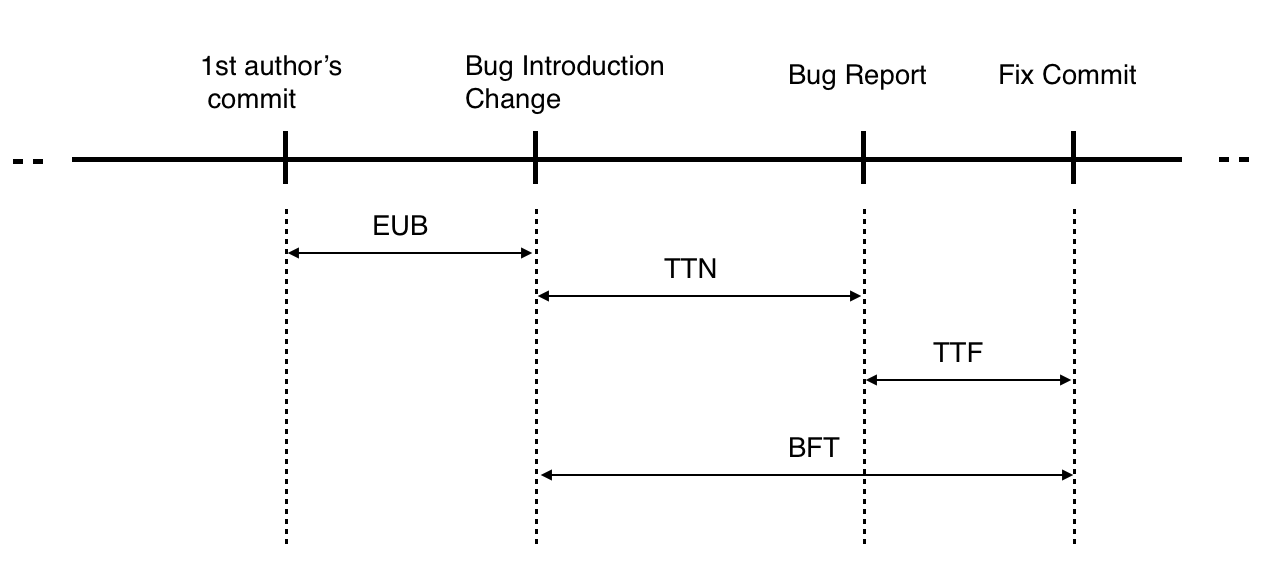
\includegraphics[width=\columnwidth]{metrics.png}
\caption{metrics}
\label{fig:graph6}       % Give a unique label
\end{figure}

\begin{figure}[ht]
\centering
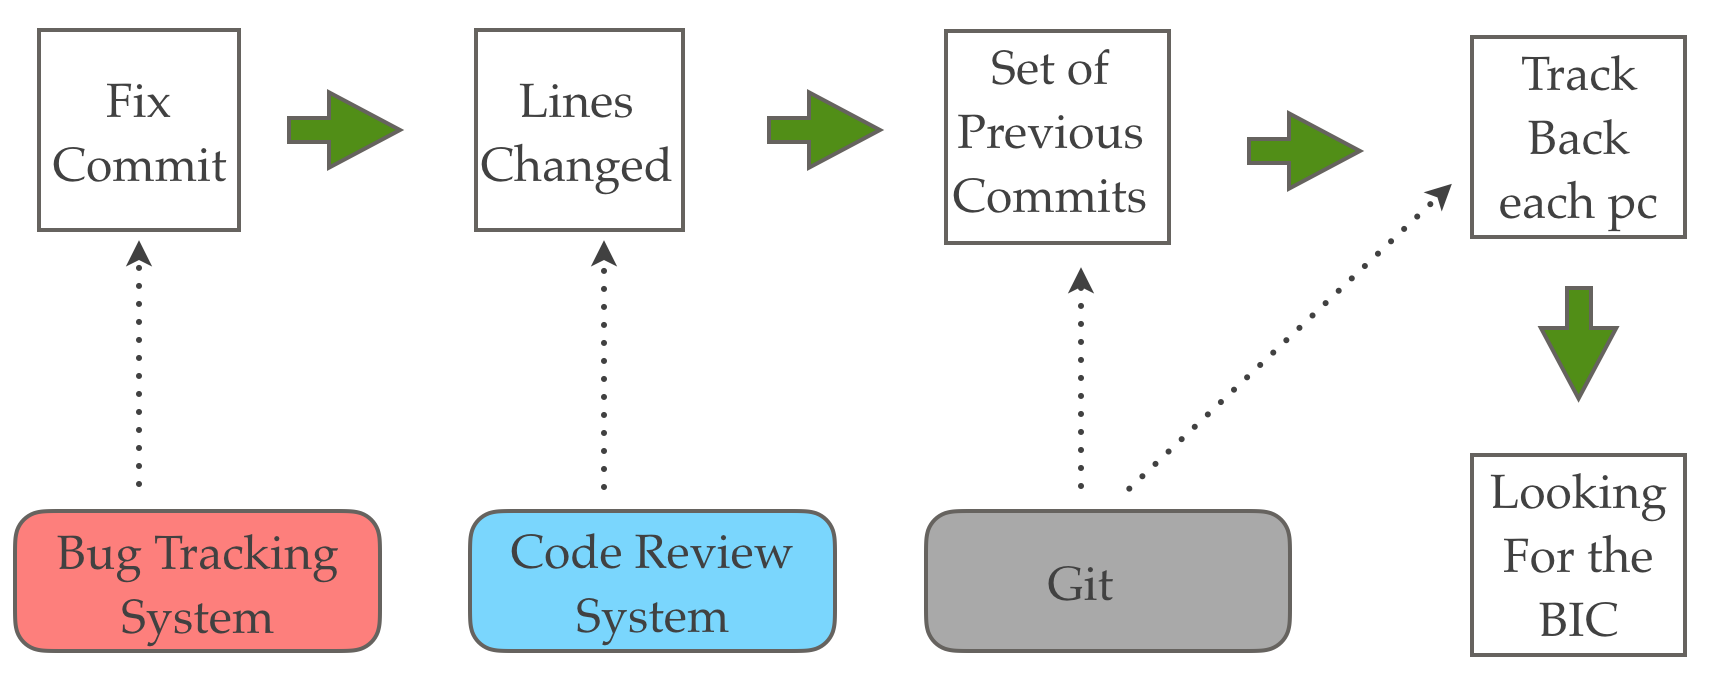
\includegraphics[width=\columnwidth]{methodology.png}
\caption{methodology}
\label{fig:graph6}       % Give a unique label
\end{figure}
- Explain how locate the BIC and the metrics that we have extracted after the BIC was found.

\section{Evaluation}
\label{sec:evaluation}
We have validated our methodology analyzing the tickets from two different projects written in different programming languages. Nova uses a dynamic language whereas ElasticSearch uses a statically language. Thus, we may study the dependency of the results with the programming language that the project is using.

In one hand, Nova belongs to OpenStack project which is a cloud computing platform with a huge developing community (more than 5,000 developers) and significant industrial support from several major companies such as Red Hat, Intel, IBM, HP, etc. The source code of Nova is written in Python and was particularly of interest because it is continuously evolving due to its very active community. Currently it has more than 44,000 commits with more than 2 million lines of code and around 1,000 contributors \footnote{\url{http://activity.openstack.org/dash/browser/repository.html?repository=nova.git&ds=scm}}. All its history is saved and available in a version control system\footnote{\url{https://wiki.openstack.org/wiki/Getting_The_Code}}, as well as its issue tracking system (Launchpad\footnote{\url{https://launchpad.net/openstack}}) and the source code review system (Gerrit\footnote{\url{https://review.openstack.org/}}). 

On the contrary, ElasticSearch is a distributed open source search and analytics engine written in Java. In spite of it has less number of commits and contributors than OpenStack, 26,000 commit and 764 contributors, its policy of label an issue as bug report is very strict, thus we could be sure that the tickets analyzed are real bug reports. Furthermore, all its code is hosted at GitHub\footnote{\url{https://github.com/elastic/elasticsearch/}}, as well as its issue list is available on GitHub\footnote{\url{https://github.com/elastic/elasticsearch/issues}}


For these two projects we analyzed the tickets looking for their trueBIC, trying to determinate if the previous commit to the fix of the ticket is a BIC. The first stage was only used in Nova due to Launchpad does not distinguish bug reports from other issues as ElasticSearch does it with its strong policy of bug label in GitHub. Thus, two different researchers, were involved in this stage, resulting that each ticket was analyzed by both researchers independently. The second stage was done manually by the first author discussing some difficult situations with two of the authors.

\section{Results}
\label{sec:results}
- TTN
- TTN vs TTN(SZZ)
- Correlation TTN with other metrics
- Plots and graphs

\begin{figure}[ht]
\centering
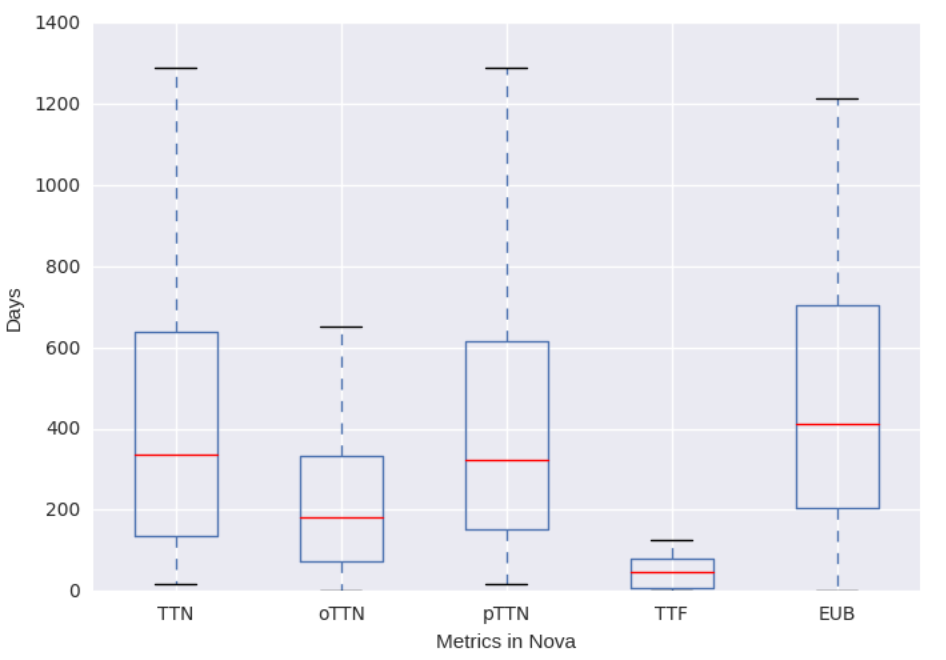
\includegraphics[width=\columnwidth]{boxplotNova.png}
\caption{BoxPlot in Nova}
\label{fig:graph4}       % Give a unique label
\end{figure}

\begin{figure}[ht]
\centering
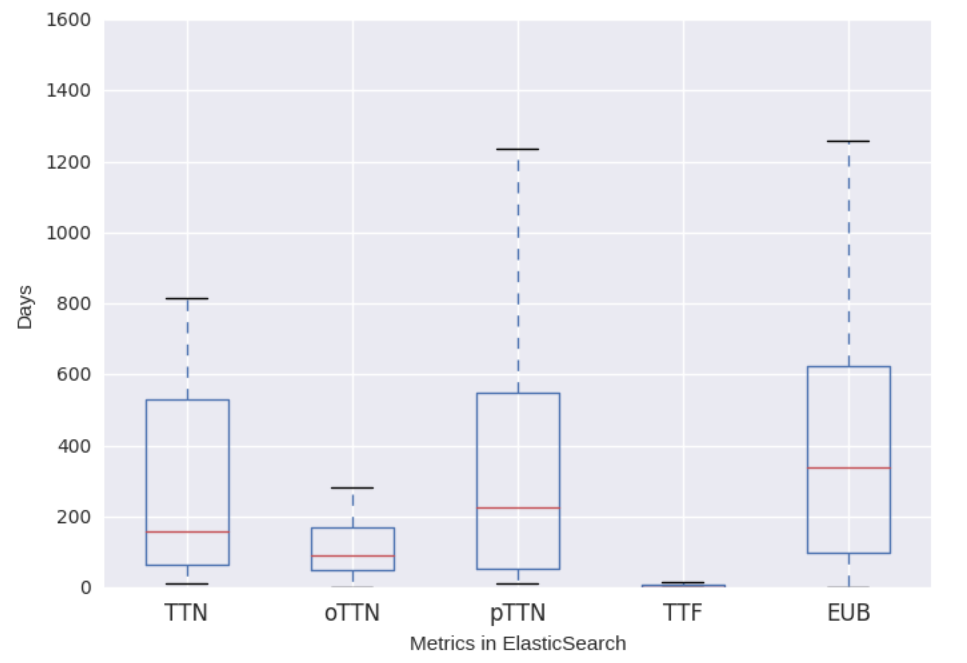
\includegraphics[width=\columnwidth]{boxplotES.png}
\caption{BoxPlot in ES}
\label{fig:graph5}       % Give a unique label
\end{figure}

\begin{figure}[ht]
\centering
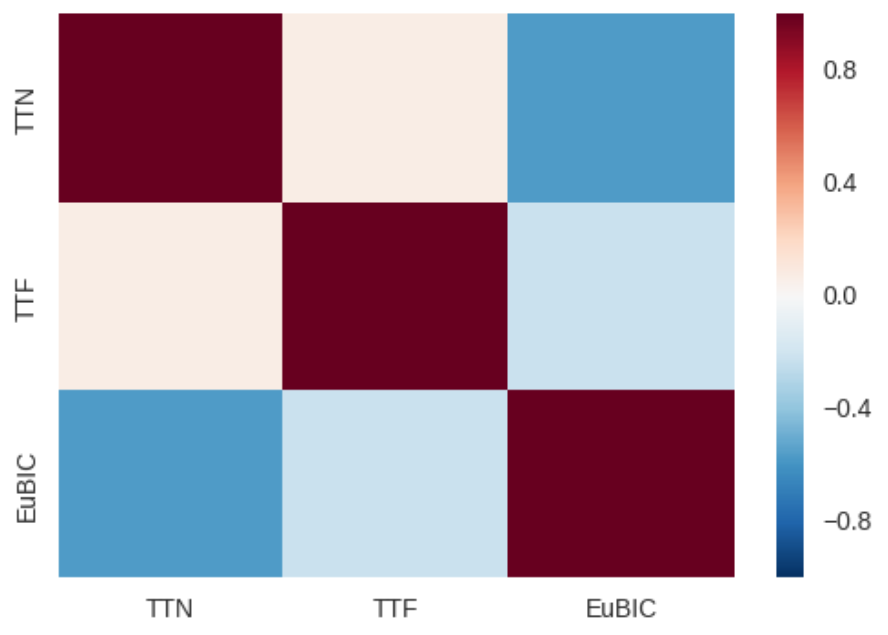
\includegraphics[width=\columnwidth]{correlationMatrix.png}
\caption{Correlation Matrix of each metric in Nova project}
\label{fig:graph}       % Give a unique label
\end{figure}

\begin{figure}[ht]
\centering
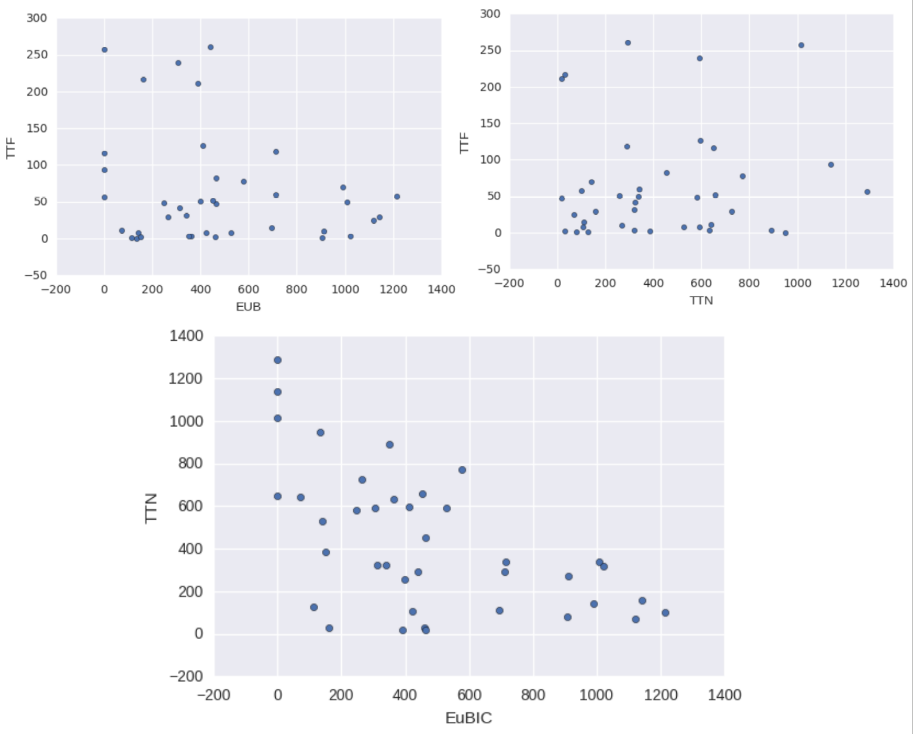
\includegraphics[width=\columnwidth]{DistributionNova_b.png}
\caption{Distribution of the metrics in Nova project}
\label{fig:graph2}       % Give a unique label
\end{figure}

\begin{figure}[ht]
\centering
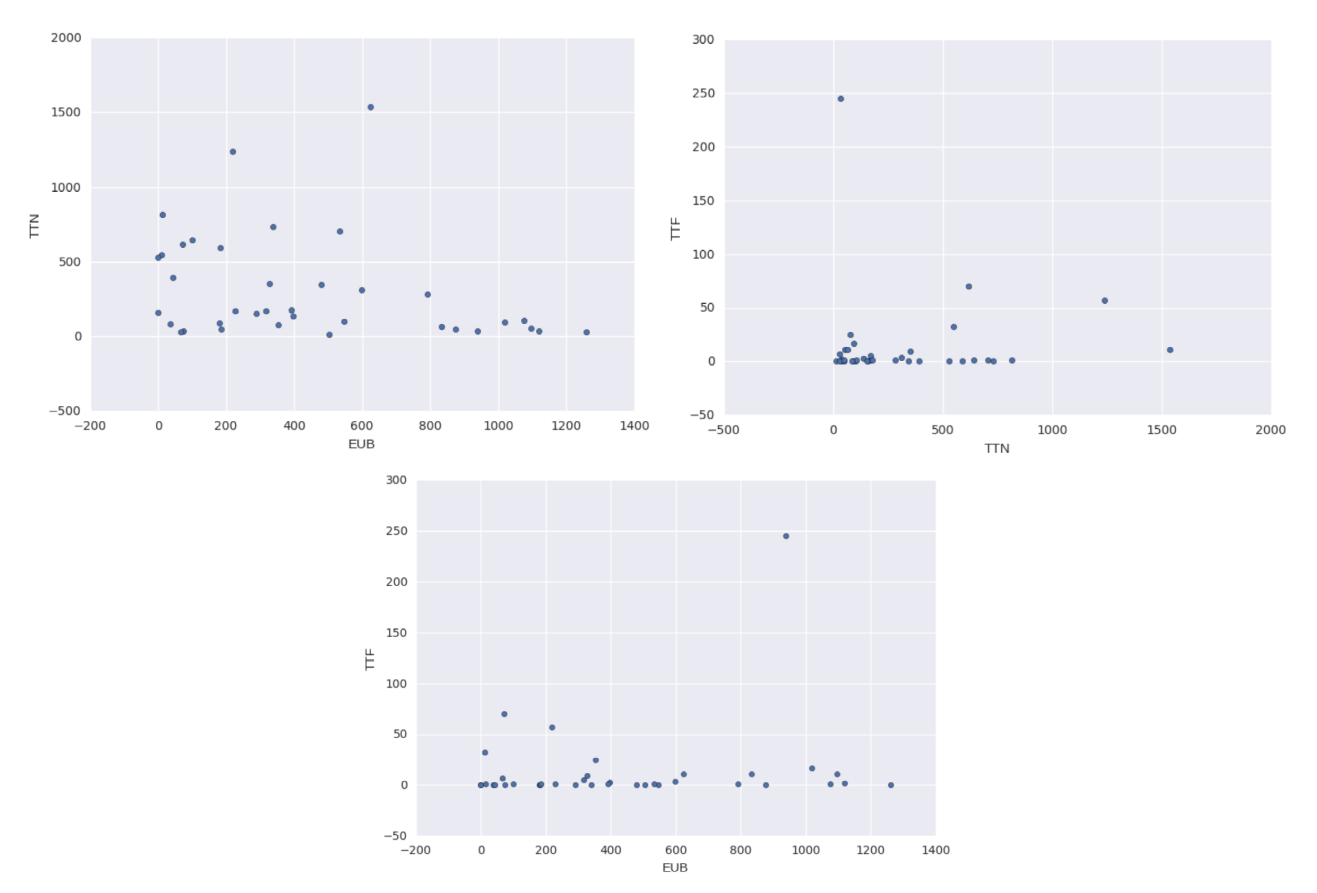
\includegraphics[width=\columnwidth]{DistributionES_b.png}
\caption{Distribution of the metrics in Nova project}
\label{fig:graph3}       % Give a unique label
\end{figure}

\begin{table}[!t]
% increase table row spacing, adjust to taste
\renewcommand{\arraystretch}{1.3}
\label{tableI}
\centering
\caption{Mean in days of the TTN, TTN\_o, TTN\_p and TTF in each project}
% Some packages, such as MDW tools, offer better commands for making tables
%% than the plain LaTeX2e tabular which is used here.
\begin{tabular}{|c||c||c||c||c| }
\hline
  & TTN & TTN\_o & TTN\_p & TTF \\
\hline
Nova & 431 & 257 & 410 & 64 \\
\hline
ElasticSearch & 312 & 171 & 375 & 14\\
\hline
\end{tabular}
\end{table}


\section{Discussion}
\label{sec:discussion}
- Possibles explanations for the TTN according to the results and have into account the other metrics


\section{Threats to validity}
\label{sec:threats}

- Small data.
- OpenSatck is continuously evolving 



\section{Conclusion}
\label{sec:conclusions}


\section*{Acknowledgment}


We want to express our gratitude to Bitergia\footnote{\url{http://bitergia.com/}} for their open source tools to mining the repositories of the projects and the support they have provided when questions have arisen. Also, we acknowledge the Spanish Government, because some authors are funded in part by it, through project TIN2014-59400-R as well as the University the Victoria and University Rey Juan Carlos that have promoted the collaboration between Universities.

% trigger a \newpage just before the given reference
% number - used to balance the columns on the last page
% adjust value as needed - may need to be readjusted if
% the document is modified later
%\IEEEtriggeratref{8}
% The "triggered" command can be changed if desired:
%\IEEEtriggercmd{\enlargethispage{-5in}}

% references section

% can use a bibliography generated by BibTeX as a .bbl file
% BibTeX documentation can be easily obtained at:
% http://www.ctan.org/tex-archive/biblio/bibtex/contrib/doc/
% The IEEEtran BibTeX style support page is at:
% http://www.michaelshell.org/tex/ieeetran/bibtex/
%\bibliographystyle{IEEEtran}
% argument is your BibTeX string definitions and bibliography database(s)
%\bibliography{IEEEabrv,../bib/paper}
%
% <OR> manually copy in the resultant .bbl file
% set second argument of \begin to the number of references
% (used to reserve space for the reference number labels box)
%\begin{thebibliography}{1}

%\bibitem{IEEEhowto:kopka}
%H.~Kopka and P.~W. Daly, \emph{A Guide to \LaTeX}, 3rd~ed.\hskip 1em plus
%  0.5em minus 0.4em\relax Harlow, England: Addison-Wesley, 1999.

%\end{thebibliography}
\newpage

\bibliographystyle{abbrv}
\bibliography{sigproc} 


% that's all folks
\end{document}


